\documentclass[12pt]{article}

\usepackage{graphicx}
\usepackage{fancyhdr}
\usepackage{rotating}
\usepackage{xcolor}
\usepackage{listings}
\usepackage{indentfirst}
\usepackage{float}
\usepackage{url}
\usepackage[margin=1in]{geometry}


\setlength{\parskip}{\baselineskip}%

\lstset{basicstyle=\ttfamily,
  showstringspaces=false,
  commentstyle=\color{red}
  keywordstyle=\color{blue}
}

\title{CS 751: Introduction to Digital Libraries - Assignment 2}
\author{Jessica McConnell}
\date{\today}

\begin{document}
\maketitle

\section{Q1}

We were required to pick 100 URIs and get WARC files for them using 4 different methods.  The methods were WARCreate, WAIL, webrecorder and wget.  We were then supposed to replay some WARC files using webrecorder and the wayback machine.

\subsection{Picking the URIs}

To get my 100 URIs I wrote a python script `pickuris.py' that picked a random number.  It then checked the size of the previously downloaded body from assignment 1. If the size of the body was more than 20,000 we used it as one of our URIs.  I picked this number by picking several different sizes and browsing to them in my web page.  At this size, the web pages started looking more intricate.

For each of the URIs I created a directory with 4 subdirectories associated with each of different methods we were supposed to use.

These URIs and associated folder number were placed in the `urissort' file.

\subsection{WGET}

I wrote a shell script to perform my wgets on all the URIs.  This script is called `wgetcommand'

WGET was the fastest method of getting the WARC files.

WGET appeared to be consistently the smallest file type.

\begin{center}
\noindent SUM:  57950068\\
LENGTH:  100\\
MEAN:  579500.68\\
MEDIAN:  41694.5
\end{center}

\subsection{webrecorder}

Webrecorder was the second tool I used to get the WARC files.  At first I maded the mistake of not erasing the previous file and kept getting WARC files for a playlist of URIs.  After figuring that out this tool was very simple.

I was not able to get a WARC file for every URI I attempted to use with this tool. I skipped these URIs for this method.

\url{http://www.louisianamusicfactory.com/shop/compact-disc/various-artists-modern-brass-band-first-second-line-in-new-orleans-1990-2005-3cds/} would not load in webrecorder.

\url{http://loveofmusicblog.blogspot.com/p/clothing.html} would cause Chrome to crash saying the site was unresponsive although it would load most of the page before crashing.

\url{https://bhamqmm.files.wordpress.com/2015/01/qmm-winter-2014.pdf} would cause a `Temporary Warc Error' whenever I tried to download the WARC.

The webrecorder files were about twice the size of the files from wget.

\begin{center}
\noindent SUM:  176759581\\
LENGTH:  97\\
MEAN:  1822263.7216494845\\
MEDIAN:  1005967
\end{center}

\subsection{WARCreate}

WARCreate was very difficult to use.  It would lock up very often.  It would also, seemingly at random times, start failing downloads saying `Failed - No File'.  The only way to resolve either of these issues was to close Chrome, open task manager and kill all processes associated with Chrome.  After that I could start downloading WARCs again.

I was also not able to get a WARC for every URI I tried with this method. In these instances of failure I would click `Generate WARC' wait for several minutes and nothing ever downloaded. These URIs were:

\noindent \url{https://bhamqmm.files.wordpress.com/2015/01/qmm-winter-2014.pdf}\\
\url{https://www.etsy.com/shop/stationeryCiaffi?utm_source=Twitter&utm_medium=PageTools&utm_campaign=Share}\\
\url{http://www.careersinconstruction.com/job/842929/quantity-surveyor-/?TrackID=17}\\
\url{http://solarsystem.nasa.gov/missions/profile.cfm?Sort=Alpha&Alias=Surveyor%2003&Letter=S&Display=ReadMore}\\
\url{http://dg-di.us/OM/FR/613029.htm}\\
\url{http://www.louisianamusicfactory.com/shop/compact-disc/various-artists-modern-brass-band-first-second-line-in-new-orleans-1990-2005-3cds/}\\
\url{http://www.iol.co.za/motoring/f1-grand-prix/ferrari-reveals-new-f1-race-car-1.1811434?utm_medium=twitter&utm_source=twitterfeed}

The WARCreate files were by far the largest files.  They were about 4 times as large as the webrecorder files and 8 times as large as the wget files.

\begin{center}
\noindent SUM:  976675632\\
LENGTH:  93\\
MEAN:  10501888.516129032\\
MEDIAN:  9785880
\end{center}

\subsection{WAIL}

I was unable to get WARC files using WAIL.  Everytime I tried to use it the application would lock up and get itself into a not responding state.

\begin{figure}[H]
    \caption{Failed WAIL}
    \centering
    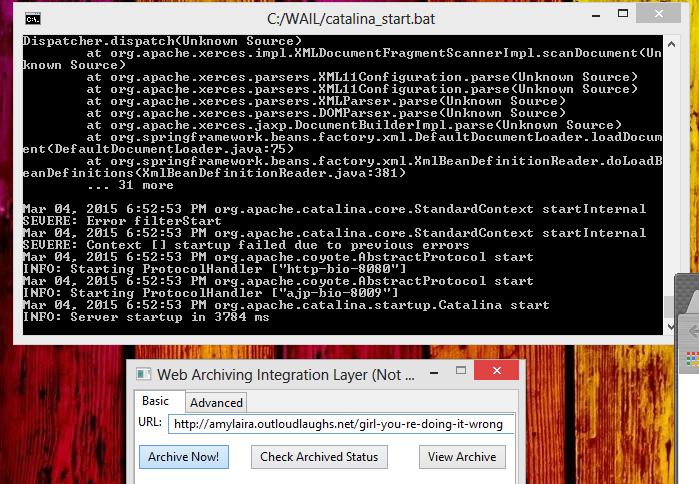
\includegraphics{failwail.PNG}
\end{figure}

\subsection{Statistics}

\begin{figure}[H]
    \caption{Mean and Median of the different methods}
    \centering
    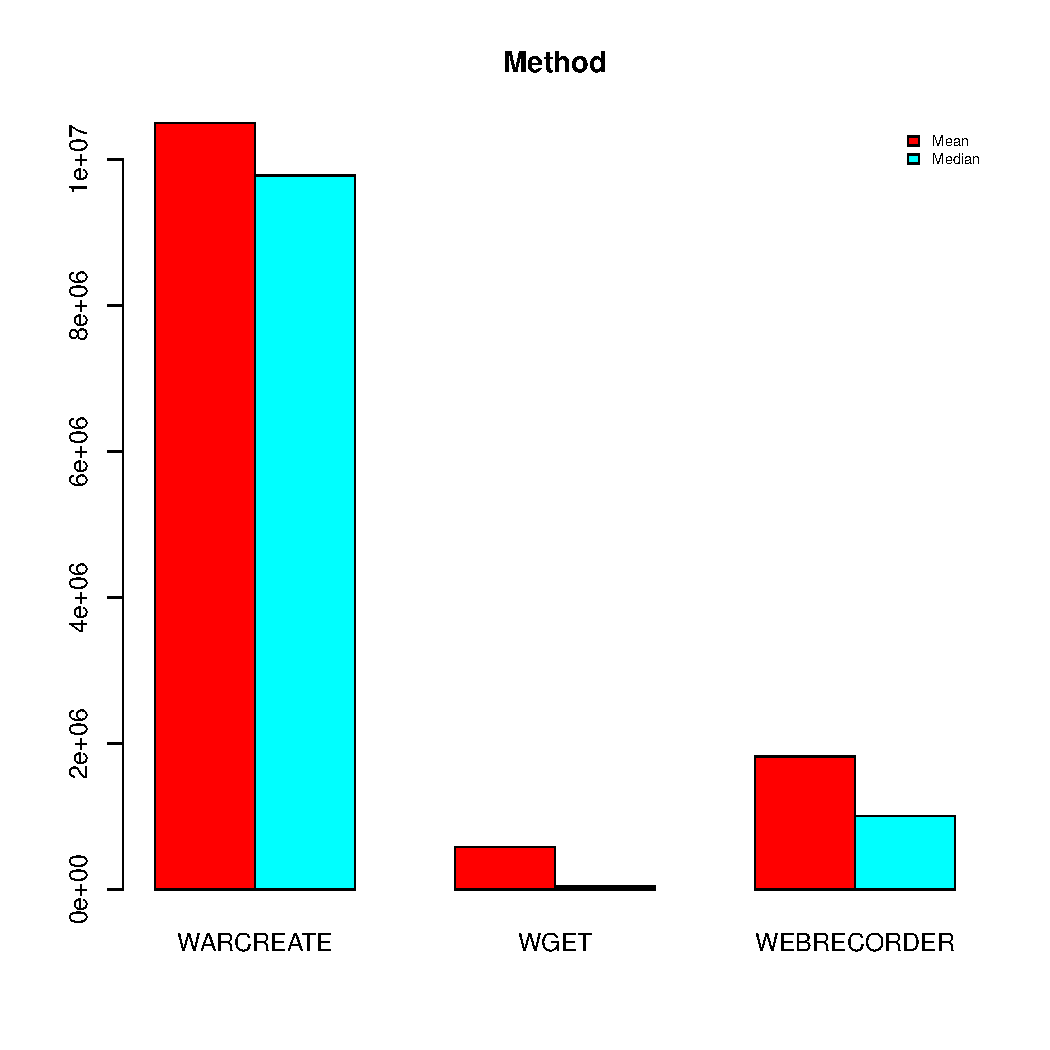
\includegraphics{sizeStats.pdf}
\end{figure}

\begin{figure}[H]
    \caption{Number of successful WARCs}
    \centering
    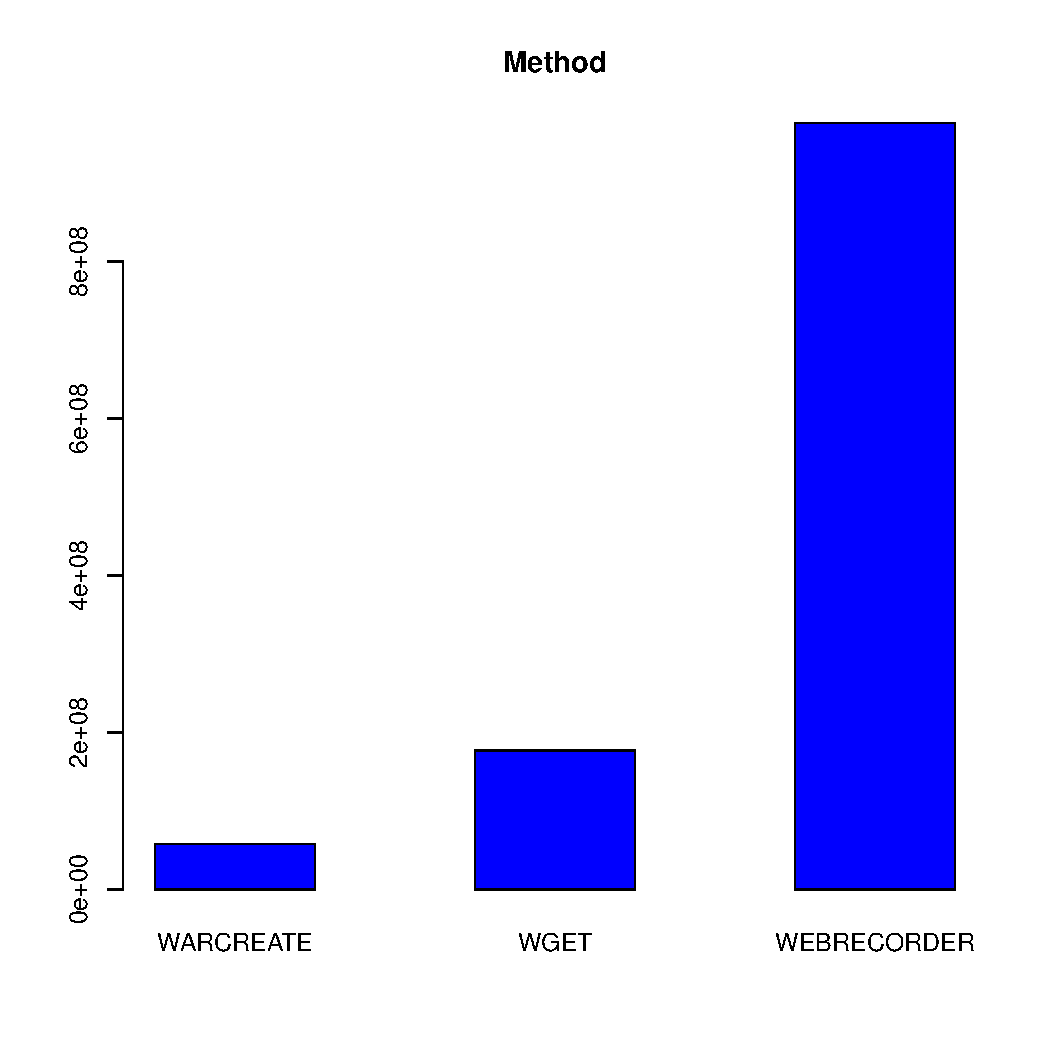
\includegraphics{warcstats.pdf}
\end{figure}

\subsection{Playback}
I chose to playback 3 WARC files.  The WARCs I chose can be found in the report directory of this folder.  In my playback I downloaded a new WARC of the replay.  During the replay some images appeared to be smaller, but otherwise everything seemed the same as when I first loaded the page.

\begin{figure}[H]
    \caption{URI number 6826}
    \centering
    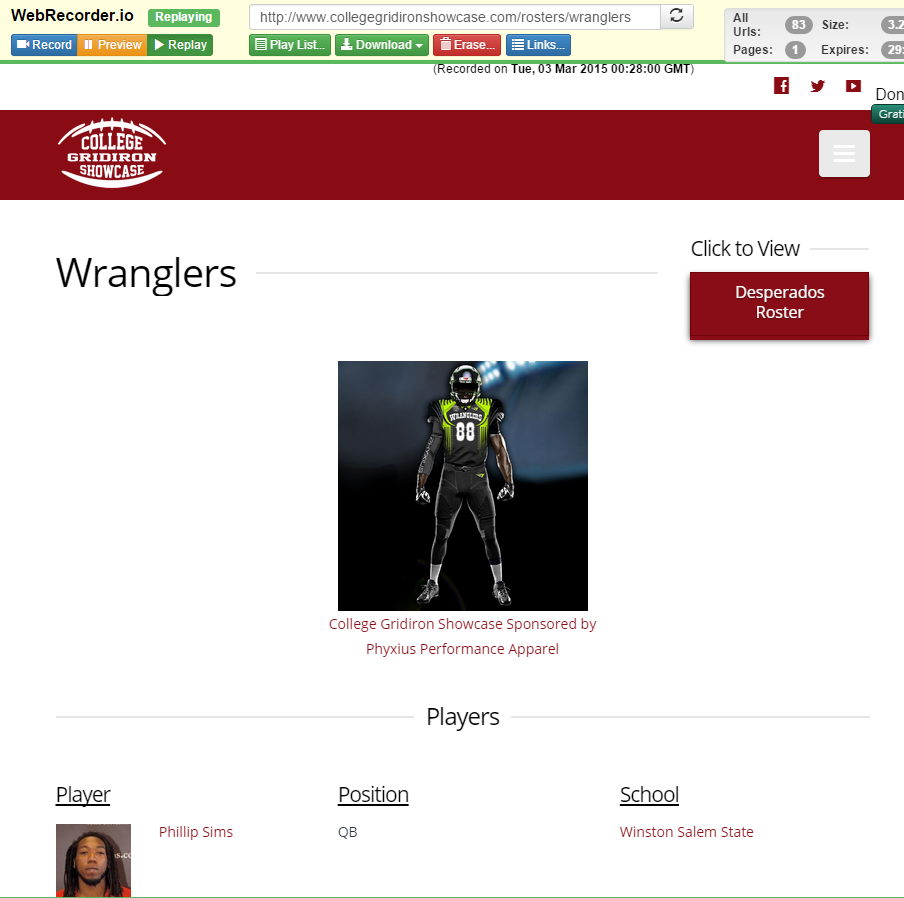
\includegraphics[scale=0.5]{collegegridironreplay.PNG}
\end{figure}

\begin{figure}[H]
    \caption{URI number 1920}
    \centering
    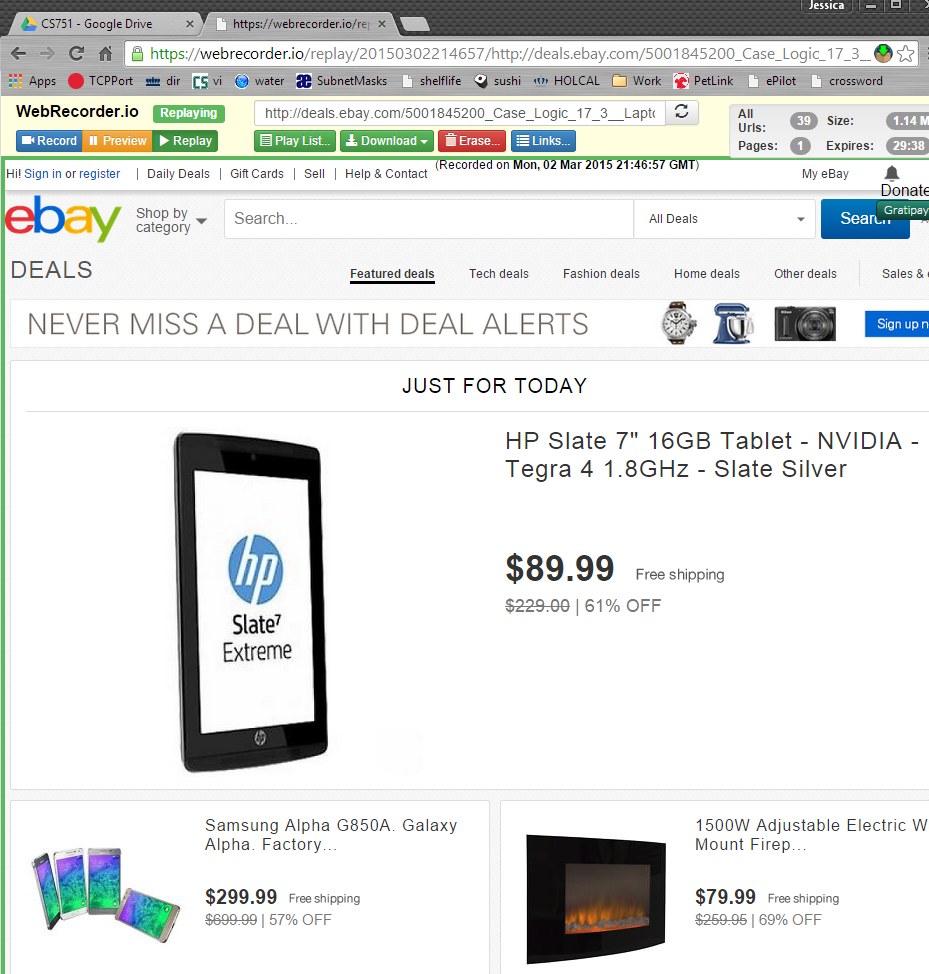
\includegraphics[scale=0.5]{ebaydealsreplay.PNG}
\end{figure}

\begin{figure}[H]
    \caption{URI number 3444}
    \centering
    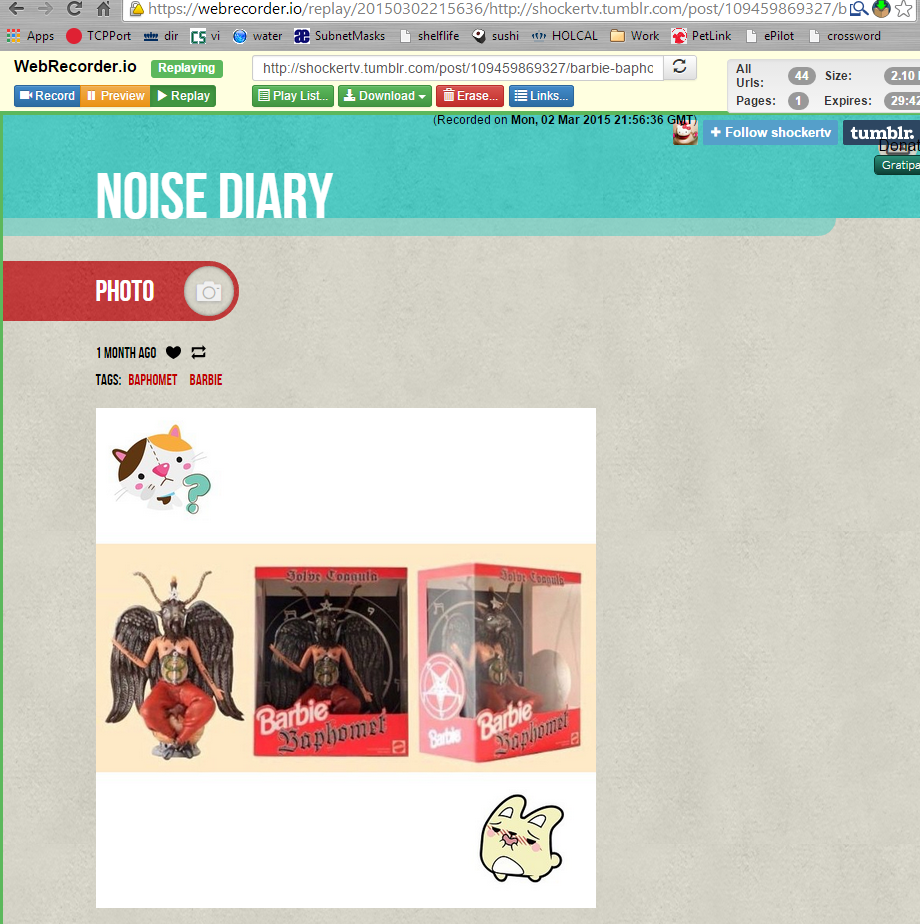
\includegraphics[scale=0.5]{shockertvreplay.PNG}
\end{figure}

I was unable to replay WARC files using WAIL.  Everytime I tried to use it the application would lock up and get itself into a not responding state.

\begin{figure}[H]
    \caption{Failed WAIL Wayback}
    \centering
    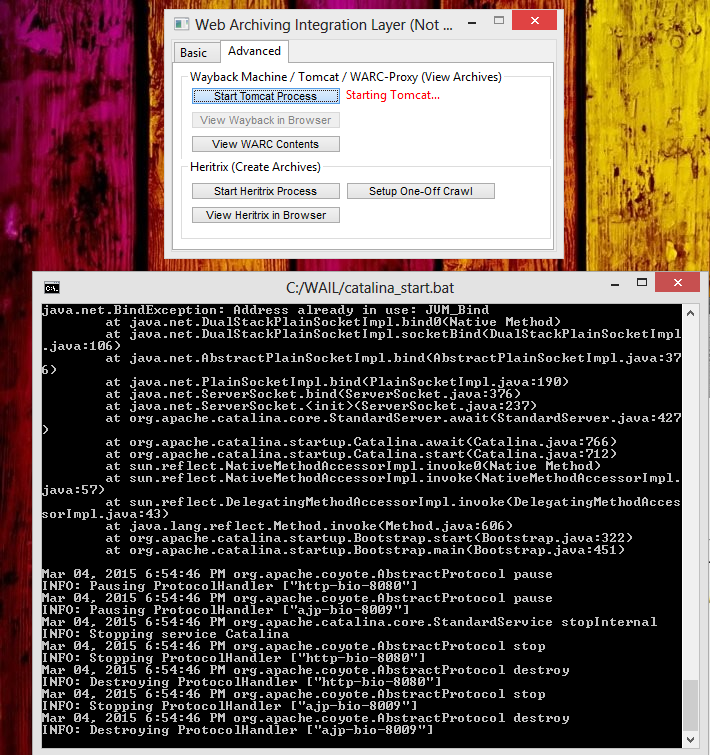
\includegraphics{failwayback.PNG}
\end{figure}



\section{Q2}

For this question we were required to build a SOLR instance, ingest 100 URIs and search.

\subsection{Setting up SOLR}

I followed got SOLR from \url{https://github.com/ukwa/webarchive-discovery} and followed the instructions at its wiki.  I was required to also install Maven.  I got the binary version from \url{http://maven.apache.org/download.cgi}.

I did not do any special confiurations for my SOLR instance. Running the server from linux.cs.odu.edu did require me to use the -Djetty.port option to change the port from 8080 to something between 10000 and 11000.

\subsection{Ingesting WARCs}
I noticed when ingesting my warc files a few of them hit the word limit and quit ingesting more words from that document.

I chose to use the WARCs received when using WARCreate due to their size. I thought it would give me more words to ingest and search on.  Here is my index stats after importing all the WARCs.

\begin{figure}[H]
    \caption{Indexes}
    \centering
    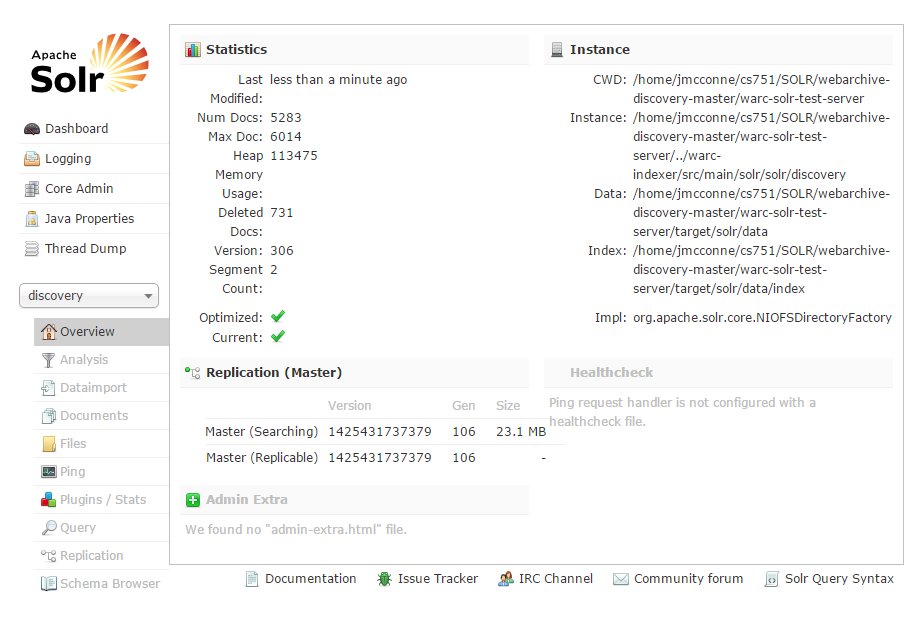
\includegraphics[scale=0.5]{indexes.PNG}
\end{figure}

\subsection{Querying}

I performed five queries.  I was surprised when it worked so well! I knew that I had a WARC file that included a web page that used the word `tennis'.  To test out querying while still ingesting the WARCs, I searched for `tennis'. As it turns out there was more files than that one that also said `tennis'.

\begin{figure}[H]
    \caption{TENNIS}
    \centering
    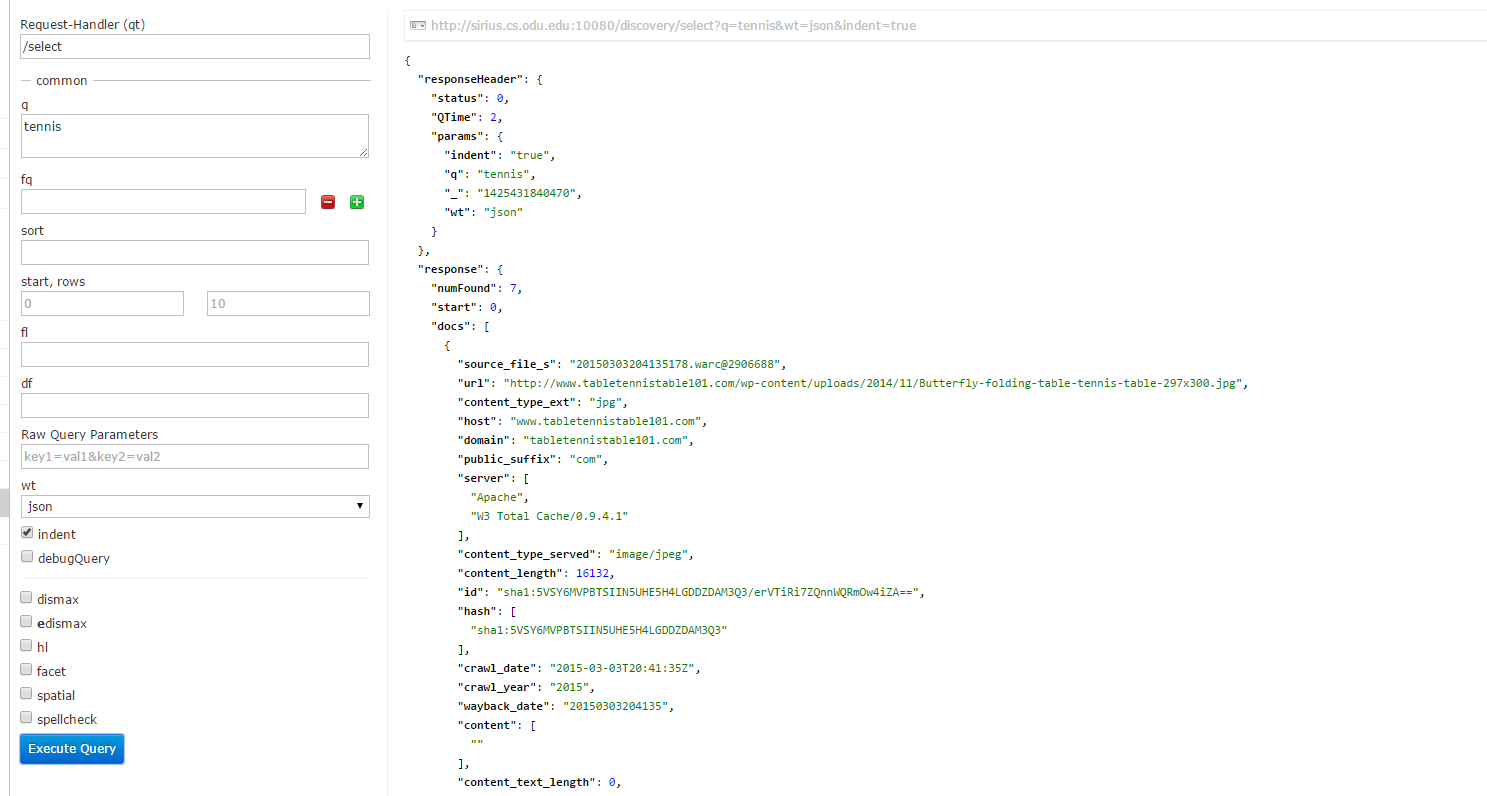
\includegraphics[scale=0.5]{tennis.PNG}
\end{figure}

After ingesting the rest of my WARC files I began searching for random words.

\begin{figure}[H]
    \caption{CAR}
    \centering
    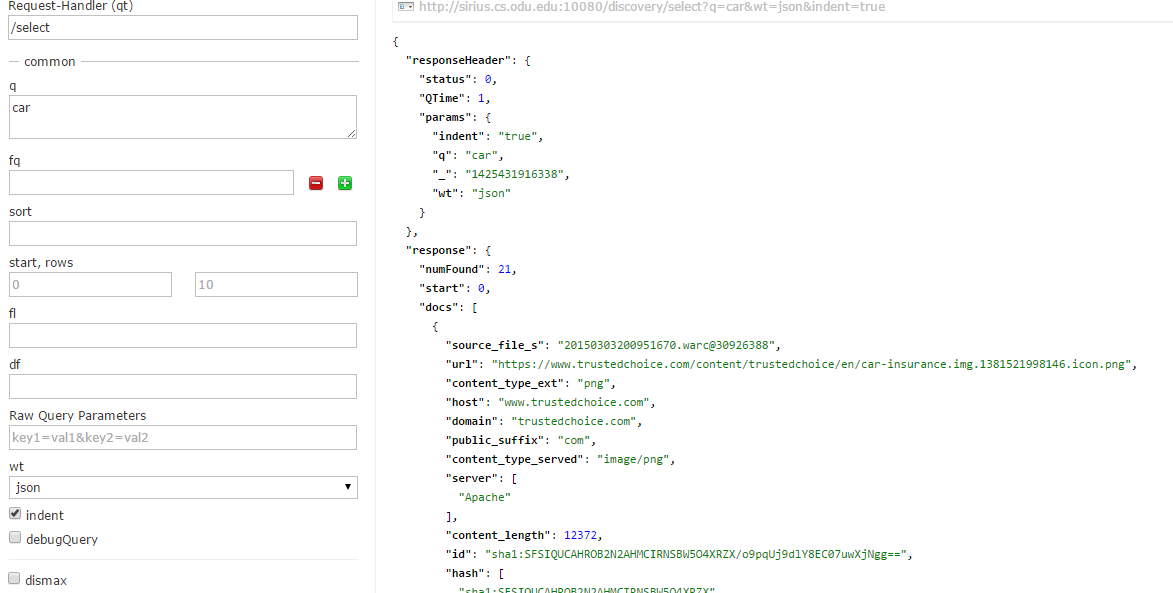
\includegraphics[scale=0.5]{car.PNG}
\end{figure}

\begin{figure}[H]
    \caption{CAT}
    \centering
    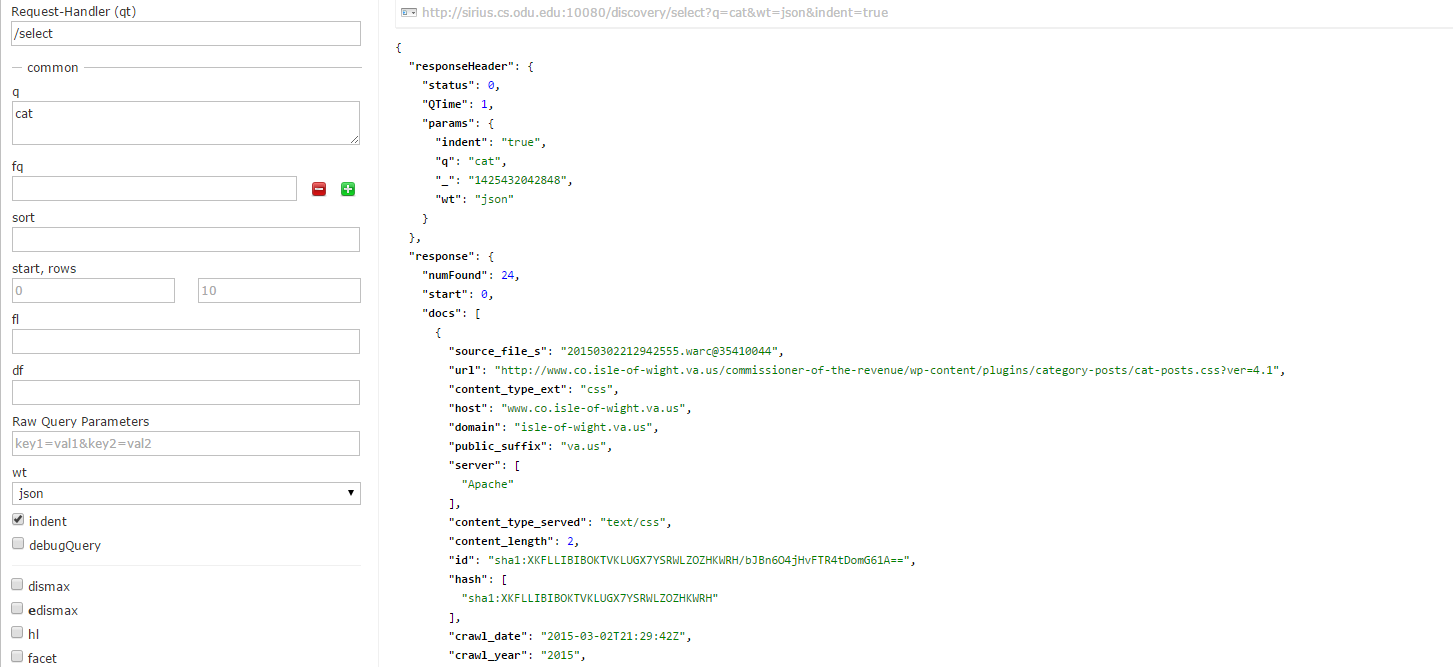
\includegraphics[scale=0.5]{catquery.PNG}
\end{figure}

\begin{figure}[H]
    \caption{MUSIC}
    \centering
    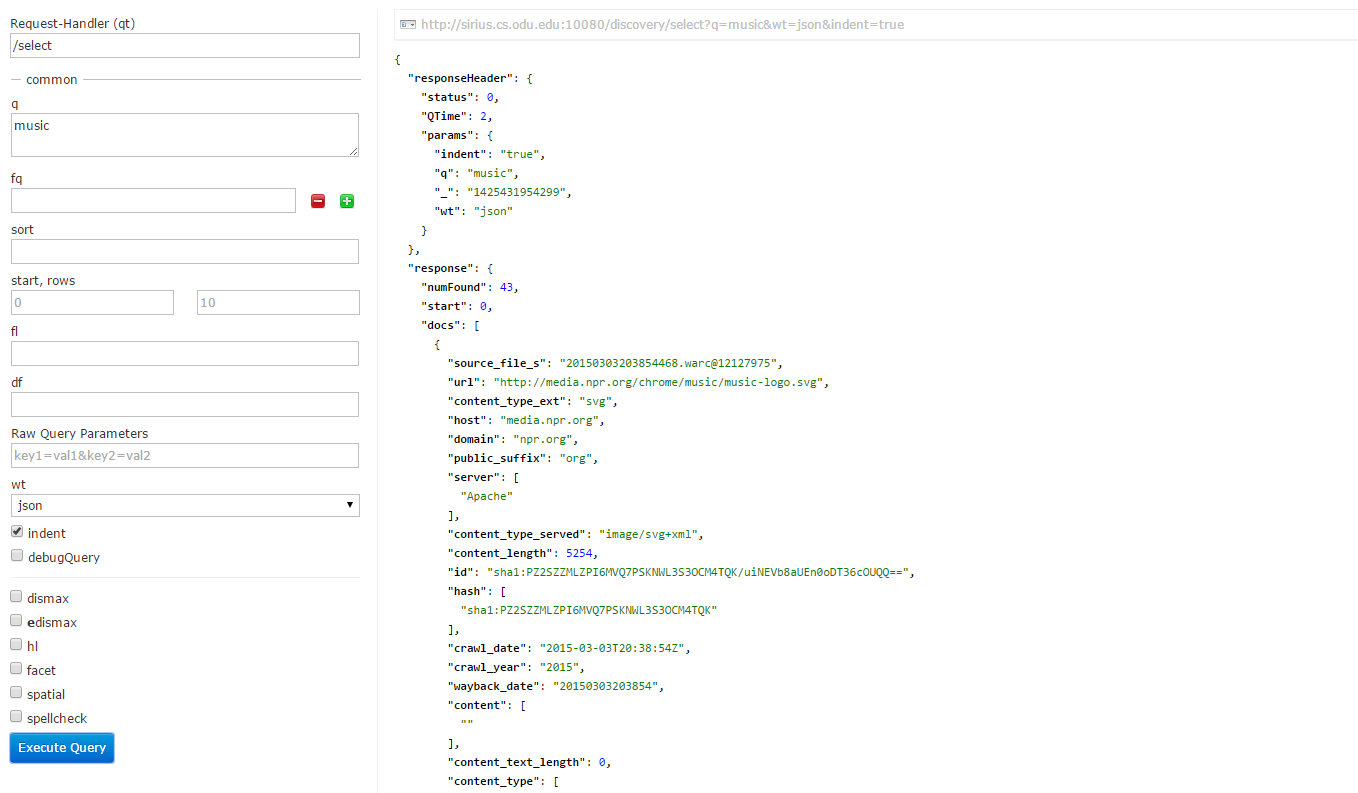
\includegraphics[scale=0.5]{music.PNG}
\end{figure}

\begin{figure}[H]
    \caption{WASHINGTON}
    \centering
    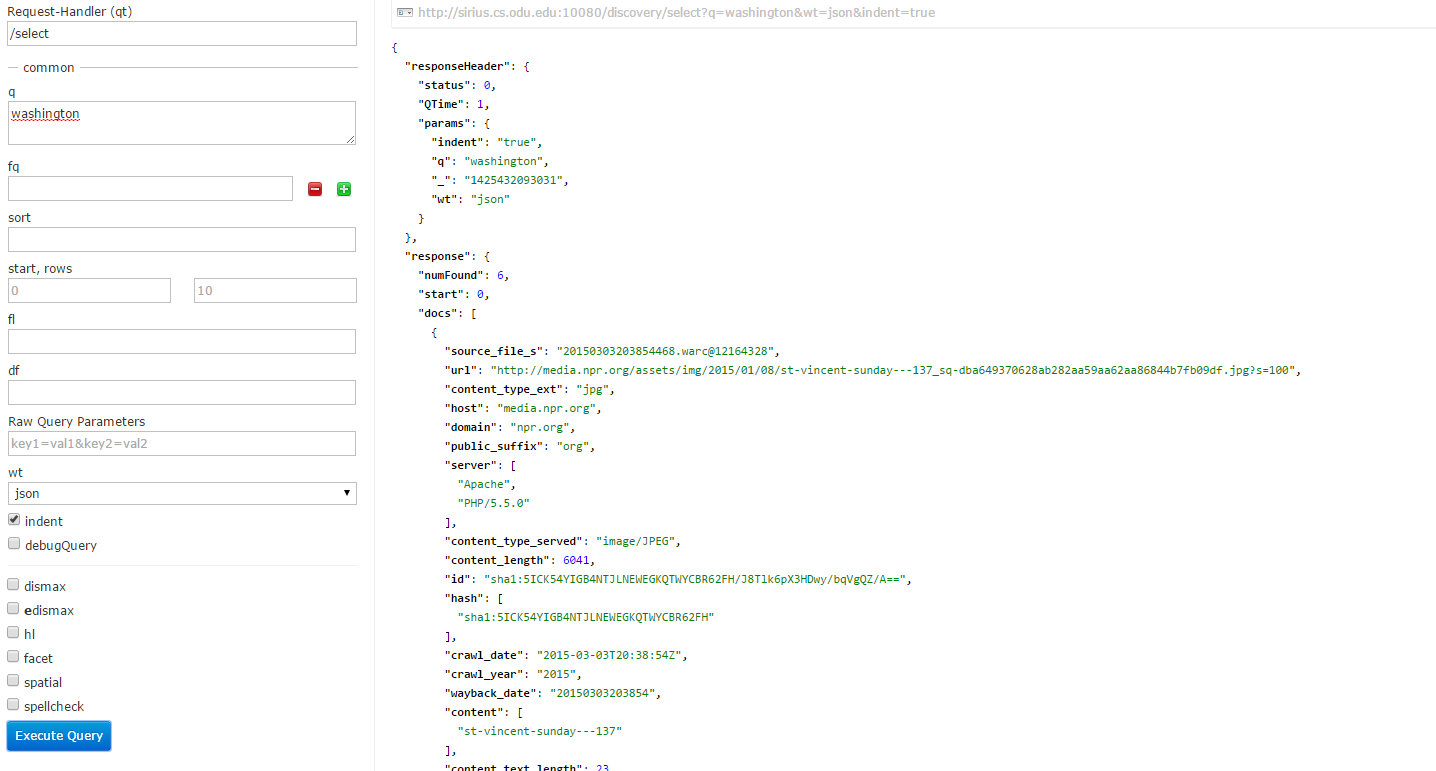
\includegraphics[scale=0.5]{washingtonquery.PNG}
\end{figure}

All of the JSON responses for these queries can be found in the report folder in files named \textit{word}query.txt.

\end{document}
